\documentclass{article}

\usepackage{amsmath}
\usepackage{url}
\usepackage{graphicx}
\usepackage{float}
\usepackage{theorem}
\usepackage[a4paper, margin=1.5in]{geometry}
\usepackage{amssymb}

\theoremstyle{definition}
\newtheorem{definition}{Definition}[section]

\renewcommand{\Re}{\operatorname{Re}}
\renewcommand{\Im}{\operatorname{Im}}
\newcommand{\reals}{\mathbb{R}}

\title{Moments and Characteristic Functions\\Instructor's Notes}
\author{Fu Tianwen \and Yao Chaorui \and Zhao Feng}

\begin{document}
	
\begin{titlepage}
	\maketitle
\end{titlepage}
\tableofcontents
\clearpage
\section{Moments}
\subsection{Definition of Moments}
Generally, in math, the $n$-th moment of a real-valued continuous function about center $c$ is: \cite{wiki:moment}
$$
\mu_n=\int_{-\infty}^\infty (x-c)^nf(x)dx
$$
In particular, for probability density functions $f$ (or cumulative density function $F$), the moments are given by
$$ \mu_n' = E[X^n] = \int_{-\infty}^\infty x^ndF(x) = \int_{-\infty}^\infty x^nf(x)dx $$
Also we have the definition of the central moment \cite{wiki:centralMoment}:
$$
\mu_n = E[(X-E[X])^n] = \int_{-\infty}^\infty (x-\mu)^nf(x)dx
$$
Generally central moments are more useful. Not to be confused with mean $\mu$.
\subsection{Description of Moments}
The first moment is the mean of a random variable, i.e. $$\mu=E[X]$$
The second moment is related to the variance of a random variable:
$$ \text{Var}[X] = E[X^2]-{E[X]}^2$$
In fact the variance is just the second central moment:
$$ \text{Var}[X] = \mu_2 = E[(X-E[X])^2]$$
As for the third central moment, a related concept is skewness. Below shows two random variables with the same mean variance however different in skewness\cite{wiki:skewness}:
\begin{figure}[H]
	\centering
	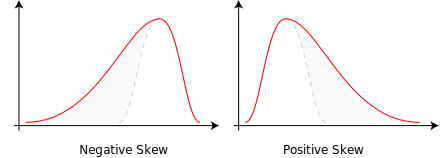
\includegraphics[width=0.8\linewidth]{img/Negative_and_positive_skew_diagrams_(English)}
	\caption{Negative and Positive Skew Diagrams} 
	\label{fig:skewness}
\end{figure}
With all moments up to the order of infinity we can describe the \textbf{characteristics} of a probability distribution.
\section{Characteristic Functions}
\subsection{Moment Generating Functions}
\begin{definition}
	Let X be a random variable with probability density function $f(x)$. If there is a positive number h such that $$ \int_{-\infty}^\infty e^{tx}f(x)dx $$
	exists and is finite for $−h < t < h$, then the function defined by
	$$M(t) = E[e^{tX}]$$
	is called the moment-generating function of $X$ (or of the distribution of $X$). 
	\textnormal{\cite{psi}}
\end{definition}
The $r$-th moment about the origin can be achieved from the moment generating function by evaluating the $r$-th derivative\cite{pennu}:
$$M^{(r)}(0) = E[X^r] $$
Also notice the relation between the Taylor Expansion and the moments.
\subsection{Characteristic Function}
Notice that $e^{tx}$ is not a "good" function in the sense that it is not bounded and may not converge under some circumstances.
Before going to characteristic functions, we first get acquainted with knowledge of complex numbers:
\subsubsection{Basic information about complex numbers}
Let $z=a+bi$, where $a,b \in \reals$, and $i=\sqrt{-1}$ is the imaginary unit. $z$ is then called a complex number and $a$, $b$ are called the real and imaginary parts of $z$, denoted by $a=\Re(z), b=\Im(z)$ respectively.
(Consider $i$ as rotation by $\frac\pi2$ counterclockwise in the complex plane)\\
The conjugate of a complex number $z=a+bi, a,b\in\reals$ is $\hat{z}=a-bi$, we also define the modulus (or length) of $z$ to be $|z|=z\hat{z}$. Notice that $|z|$ is a non-negative real number.\\
Euler's formula: $$e^{i\theta} = \cos\theta + i\sin\theta$$ The formula comes from Taylor's Series. It also gives rise to the polar representation of a complex number, i.e. $z=re^{i\theta}$, where $r$ is the modulus and $\theta$ is the phase.\\
From this we also have that $|e^{i\theta}| = 1$ for any $\theta$.
\subsubsection{Definition of Characteristic Functions}
\begin{definition}
	Let $X$ be a random variable and denote by $F$ the cumulative distribution function of $X$. The characteristic function $\varphi=\varphi_X$ of $X$ (or of $F$, in which case we also write $\varphi_F$) is defined by \textnormal{\cite{cfms}}
	$$\varphi_X(t):=E[e^{itX}]=\int_{-\infty}^\infty e^{itx}dF(x), t\in\reals$$
\end{definition}
\subsubsection{Basic Properties}
\subsection{Common Distributions and Their Characteristic Functions}
%also include some figures here
\section{Examples and Applications of Characteristic Functions}
To be continued...
\medskip

\bibliographystyle{ieeetr}
\bibliography{bibliography}
\end{document}